%%%%%%%%%%%%%%%%%%%%%%%%%%%%%%%%%%%%%%%%%
% Stylish Article
% LaTeX Template
% Version 1.0 (31/1/13)
%
% This template has been downloaded from:
% http://www.LaTeXTemplates.com
%
% Original author:
% Mathias Legrand (legrand.mathias@gmail.com)
%
% License:
% CC BY-NC-SA 3.0 (http://creativecommons.org/licenses/by-nc-sa/3.0/)
%
%%%%%%%%%%%%%%%%%%%%%%%%%%%%%%%%%%%%%%%%%

%----------------------------------------------------------------------------------------
%	PACKAGES AND OTHER DOCUMENT CONFIGURATIONS
%----------------------------------------------------------------------------------------

\documentclass[fleqn,10pt,ngerman]{SelfArx}
\usepackage{babel}
\selectlanguage{ngerman}

\setlength{\columnsep}{0.55cm} % Distance between the two columns of text
\setlength{\fboxrule}{0.75pt} % Width of the border around the abstract

\definecolor{color1}{RGB}{0,0,90} % Color of the article title and sections
\definecolor{color2}{RGB}{0,20,20} % Color of the boxes behind the abstract and headings

\newlength{\tocsep} 
\setlength\tocsep{1.5pc} % Sets the indentation of the sections in the table of contents
\setcounter{tocdepth}{2} % Show only three levels in the table of contents section: sections, subsections and subsubsections

\usepackage{comment}

\usepackage{fontenc}
\usepackage{inputenc}
\usepackage{url} 
\usepackage[hidelinks]{hyperref}
\usepackage{listings}
\usepackage{dirtree}
%----------------------------------------------------------------------------------------
%	ARTICLE INFORMATION
%----------------------------------------------------------------------------------------

\JournalInfo{Software-Technik-Praktikum} % Journal information
\Archive{Sommersemester 2019} % Additional notes (e.g. copyright, DOI, review/research article)

\PaperTitle{Implementierung von REST Services zur Umsetzung der SQLcoach Anwendung} % Article title

\Authors{Daniel Braun} % Authors
\affiliation{\textit{Hochschule Kaiserslautern}} % Author affiliation
\affiliation{\textbf{Corresponding author}: Braun Daniel} % Corresponding author

\Keywords{SQL-Coach, REST, Java, Service,Postman, Docker } % Keywords - if you don't want any simply remove all the text between the curly brackets
\newcommand{\keywordname}{Keywords} % Defines the keywords heading name

%----------------------------------------------------------------------------------------
%	ABSTRACT
%----------------------------------------------------------------------------------------

\Abstract{
Der implementierte SQLcoach stellt die Grundlage für eine webbasierte Anwendung dar, welche es Nutzern ermöglicht, ihre SQL-Kenntnisse zu prüfen, festigen oder zu erneuern. Vorbild für dieses Projekt war der 2007 unter der Leitung von Prof.Dr.Schiefer erstellte SQL-Coach, welcher hier mit neuen Methoden neu aufgesetzt wurde. Hierzu wurde ein Stammdatensatz von Szenarien, Aufgabengruppen und Aufgaben erstellt, anhand derer weitere Szenarien erstellt werden können. Methoden zum Einfügen, Entfernen, Ausgeben und Updaten wurden als Möglichkeit zur Verwaltung dieser Daten bereits implementiert. Einer der von Prof. Dr. Schiefer definierten Trainingsdatensätze \dq DATA\_Personal \dq läuft in einem Docker Container, sodass auf diesem Queries zu Testzwecken ausgeführt werden können.
Um diese Software aufzusetzen wurden verschiedene Methoden erlernt und moderne Werkzeuge wie JAX-RS verwendet, welche in Kapitel 2 genauer beschrieben werden. JAX-RS bietet eine Möglichkeit, RESTful-Services in Java zu programmieren, dessen Nutzung den Vorteil hat, dass REST viele HTTP-Methoden verwendet und die Software dadurch leicht in andere Systeme und Anwendungen zu integrieren ist. Durch die Nutzung von Docker und Git wurde gewährleistet, dass man den Code leicht bekommen und ausführen kann, sodass dieser im Nachhinein verändert werden kann. Hierdurch ist es  möglich, den SQL-Coach als
Grundlage für weitere SQL-Projekte zu verwenden oder ihn zu erweitern, wodurch  die in der Zusammenfassung formulierten Aufgabenstellungen von anderen Nutzern realisiert werden können.}

%----------------------------------------------------------------------------------------

\begin{document}
	
	\flushbottom % Makes all text pages the same height
	
	\maketitle % Print the title and abstract box
	
	\tableofcontents % Print the contents section
	
	\thispagestyle{empty} % Removes page numbering from the first page
	
	%----------------------------------------------------------------------------------------
	%	ARTICLE CONTENTS
	%----------------------------------------------------------------------------------------
	
	\newpage
	\section{Einleitung} % The \section*{} command stops section numbering
	

	
	Der SQL-Coach ist eine 2007 an der Hochschule Kaiserslautern von Christoph Gerstle und Florian Moritz unter der Leitung von Dr. Prof. Schiefer, entwickelte eLearning Plattform, welche sowohl das Üben als auch das Festigen von SQL-Requests auf einer Trainingsdatenbank ermöglicht.  Diese zwölf Jahre alte webbasierte Anwendung basiert aber auf veralteten Technologien wie das MMVC framework Apache Struts(\url{https://struts.apache.org/}) und wurde deshalb im Projekt mit aktuellen Technologien neu aufgesetzt. 
	Bei dieser neuen Implementierung wurde darauf geachtet, dass grundlegende Funktionalitäten weiterhin bestehen. Des Weiteren ist der Code in einer solchen Art und Weise aufgebaut und dokumentiert, dass es leicht ist, weitere Funktionen im Nachhinein zu ergänzen. Dies garantiert, dass der Code wartbar und erweiterbar ist.
	\newpage
	Die alte Version hatte folgende Funktionalitäten:
\begin{itemize}
	\item Die Struktur der in der Aufgabe verwendeten Tabelle wird angezeigt (Abbildung\ref{fig:fsm2})
	\item Trainingsdatensätze stehen bereit
	\item Select Queries können auf diesen Trainingsdaten ausgeführt werden
	\item das Ergebnis der vom Nutzer erstellten Query wird einer Musterlösung gegenübergestellt (Abbildung \ref{fig:fsml3})
\end{itemize}
	
	
		\begin{figure}[ht]\centering
		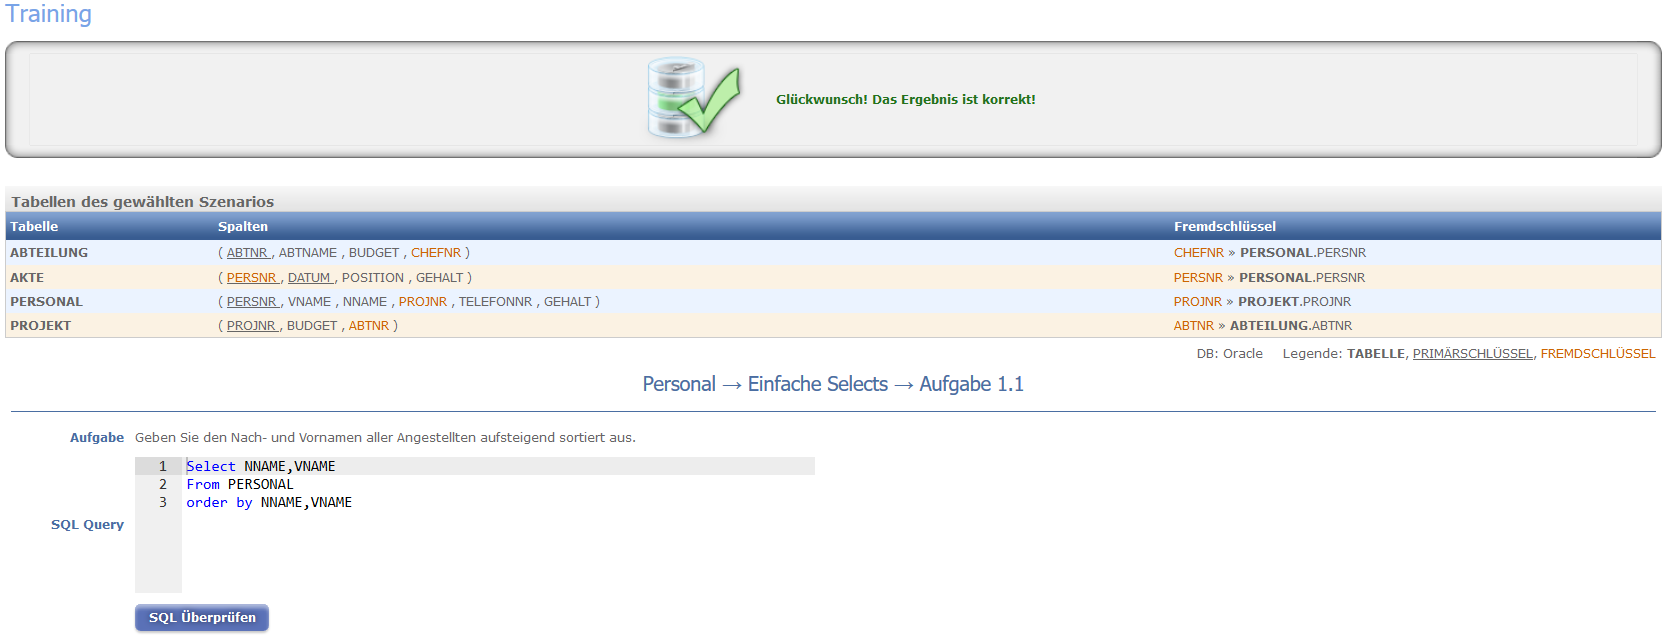
\includegraphics[width=9 cm]{Abbildungen/SQL_Coach_Aufgabe}
		\caption{Aufgabenstellung und Interface (Quelle \url{https://sqlcoach.informatik.hs-kl.de/sqlcoach/}).}
		\label{fig:fsm2}
	\end{figure}
	\begin{figure}[ht]\centering
		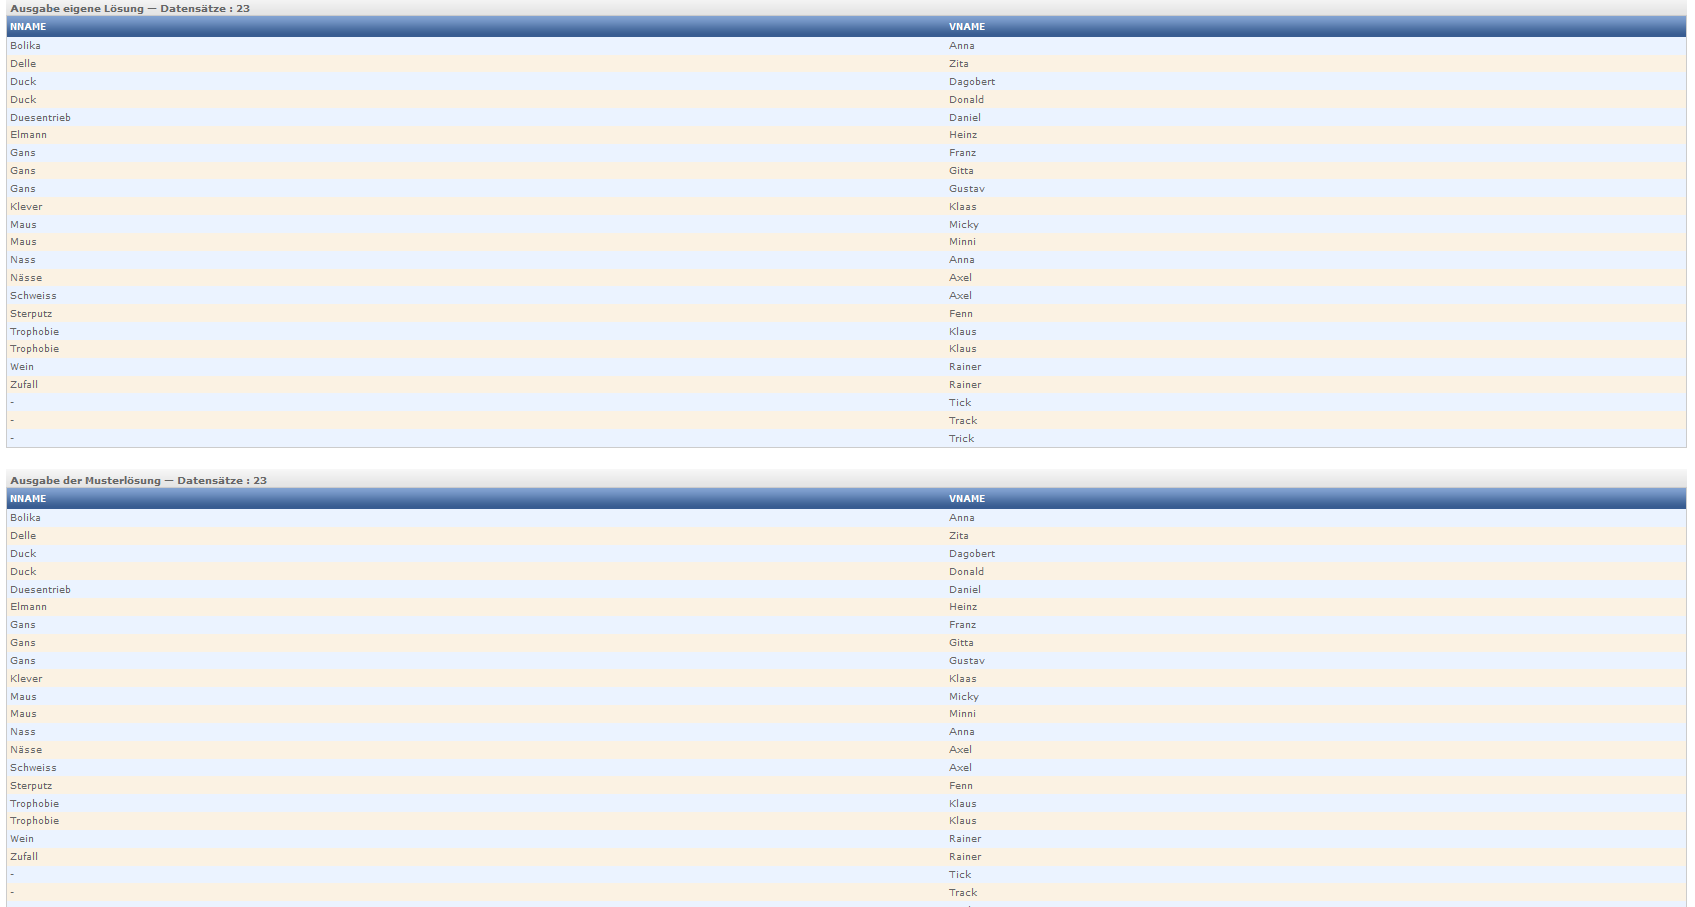
\includegraphics[width=9 cm]{Abbildungen/TabellenBild}
		\caption{Die SQLcoach Anwendung (Quelle \url{https://sqlcoach.informatik.hs-kl.de/sqlcoach/}).}
		\label{fig:fsml3}
	\end{figure}
	%------------------------------------------------

	
	
	
	
	
	
	%------------------------------------------------

	\section{Methoden und Werkzeuge}
	\label{sec:methoden}
	Um modernen Anforderungen gerecht zu werden, wurden im Projektverlauf moderne Methoden und Werkzuge genutzt, die im folgenden Abschnitt erläutert werden. Es werden außerdem die von den Werkzeugen erstellten Artefakte genannt und beschrieben.\newline 
	Kurzübersicht:
	JAX-RS wurde als Möglichkeit zur Implementierung von RESTful Web Services in Java genutzt. 
	Mit Docker und Git wurde gewährleistet, dass das Projekt leicht zu installieren und Betriebssystem unabhängig ist.
	Maven verwaltet als Build-Management-Tool den Build-Prozess der Anwendung.
	Die Datenbanken beruhen auf Postgres und Log4j wurde als Logger verwendet.
	
	
	\subsection{JAX-RS und Jersey}\label{JAX-RS und Jersey}
	JAX-RS wurde im Zuge der Tutorialreihe "REST Web Services"\footnote{\url{https://www.youtube.com/playlist?list=PLqq-6Pq4lTTZh5U8RbdXq0WaYvZBz2rbn}} als Java Programmierschnittstelle kennengelernt.
	
	\noindent REST ist ein Architekturstil, der die Kommunikation zwischen Rechnern vereinfachen soll.
	Er wird überwiegend für Webservices im Client-Server-Modell verwendet.
	Im Projekt wurden verschiedene Annotationen verwendet, unter anderem:\newline
	Pfad Annotationen, welche die Url der Schnittstelle definieren, der Requesttyp, welcher die Art der Anfrage definiert, sowie @Consumes und @Poduces, welche den MIME-Typ der jeweiligen akzeptierten bzw. zurückgegebenen Ressource definieren.
	\subsection{Docker}
	Docker  ist ein Betriebssystem unabhängiges\footnote{Damit Docker auf Windows läuft ist eine Virtualbox oder HYper-V, welches Bestandteil von Windows-Servern und Windows 8/10 in der Pro-,Enterprise- oder Educatio-edition ist,von Nöten.} Programm, welches es ermöglicht, ganze Programme in Containern zu kapseln, wodurch Portabilität und Kompatibilität garantiert werden. 
	Gemäß der Docker-Design-Vorgaben soll pro container nur ein prozess laufen, weshalb die SQLcoach-Anwendung auf einem Tomcat-Docker-Container und zwei Datenbank-Docker-Containern umgesetzt wurde. \newline
	Die Docker-Compose-Datei  docker-compose.yml \footnote{\url{https://docs.docker.com/compose/}}
	spezifiziert die drei Images für die  oben erwähnten Container. In dieser Datei werden auch die Ports, die Abhängigkeiten und die verwendeten Passwörter spezifiziert.
	Der Container für die Katalogdatenbank wird auf Basis des Images postgres:9.6-alpine erstellt. Der SQL-Coachservice wird mit \textit{docker/tomcate/dockrfile} erstellt und mit Hilfe der  \textit{init\\database.sql} initialisiert. 
	
	
	\subsection{Maven}
	Maven ist ein Java-basiertes Build-Management-Tool, welches die Abhängigkeiten beschreibt und den Build-Prozess der Anwendung verwaltet. Die pom.xml Datei beschreibt, welche Anwendungen erzeugt  und  nach der Erstellung in den Zielordner eingefügt werden.\newline
	Die folgenden Dependencies werden über die pom.xml spezifiziert:
	\begin{itemize}
		\item Jersey (Kapitel \ref{JAX-RS und Jersey})
		\item log4j	 (Kapitel \ref{log4j})
		\item hikari
		\item javax
	\end{itemize}
	\newpage
	
	\subsection{Postgres/SQL}
	Postgres wurde als objektrelationales Datenbankmanagementsystem (ORDBMS)"\footnote{\url{http://www.postgresql.de/index.whtml}} eingeführt und ersetzte somit Oracle SQL Developer, welcher für das zu verbessernde Projekt von 2007  genutzt wurde. 
	Die im Projekt verwendete und strukturbestimmende Stammdatenbank sind in der SQL-Datei init\_database.sql definiert. Der implementierte Trainingsdatensatz wurde in der davon unabhängigen Datei personaldatensatz.sql definiert.

	\subsection{Apache Log4j}\label{log4j}
	Apache Log4j ist ein Java-basiertes Hilfsprogramm, welches dem Loggen von Anwendungsmeldungen dient. 
	Apache Log4j erstellt automatisch Protokolle, welche das Finden von Fehlern erleichtern und so den Debugging-Prozess beschleunigen.
	Die Klasse \textit{SqlCoachDBFacet} initialisiert eine Protokollinstanz als Klassenattribut durch \newline\textit{private static final Logger log =\newline Logger.getLogger(SqlCoachDBFacet.class);}, wobei\newline
	\textit{getLogger(SqlCoachDBFacet.class)}\footnote{\url{https://logging.apache.org/log4j/1.2/apidocs/org/apache/log4j/Logger.html\#getLogger(java.lang.Class)}} ein Protokoll mit dem Namen der Klasse (SqlCoachDBFacet) erzeugt wird. Mit log.trace() \footnote{\url{http://logging.apache.org/log4j/1.2/apidocs/org/apache/log4j/Level.html\#TRACE}} erstellte man in der SQLCoachDBFacet-Klasse ein Protokoll, welches bei einem Fehler zurückgegeben wird und detaillierte Informationen über diesen liefert.
	
	
	
	\subsection{GIT}
	Git ist ein Filehosting-Service, der es Nutzern erlaubt,  Codes hoch- und herunterzuladen bzw. verschiedene Versionen desselben Codes zu verwalten. Durch sogenannte Branches ist es möglich, den Code auf einem alternativen Pfad unabhängig vom vorigen Projektstand weiterzuentwickeln. Diese Branches werden mit sogenannten "merges" wieder mit ihrem Parent (der Pfad, von welchem sie gebranched wurden) vereinigt, wobei Git inkompatible Codes selbstständig identifiziert und den Merge gegebenenfalls blockiert, bis der Konflikt behoben wurde und trägt somit zur Code-Integrität bei. 
	Für das Projekt wurde ein Github Repository  angelegt, in welchem sich der gesamte Sourcecode sowie die Dokumentation des Projektes befindet. Dieses Repository dient  als externes Backup und gibt anderen Nutzern die Möglichkeit, den Sourcecode zu ziehen (dies geschieht in Github mit einem sogenannten PULL-request), um den Code zu \dq reviewen"\dq oder weiterzuentwickeln. 
	
	\newpage
	\section{Ergebnisse}
In Kapitel 3.1 werden die implementierten REST-Schnittstellen aufgelistet und beschrieben. \newline In Kapitel 3.2 ist eine Installationsanleitung sowie eine Spezifikation der Installationsvoraussetzungen.\newline
In Kapitel 3.3 ist beschrieben, wie die einzelnen Methoden aus Kapitel \ref{sec:methoden} umgesetzt wurden und in welcher Relation die einzelnen Artefakte bzw. Werkzeuge stehen.
	%Endergebnisse beschreiben und Bezug auf Kap 2 nehmen
	%neutral nüchtern
	%passive nicht "ich habe oder wir haben" sondern " es wurde"

	
	\subsection{REST Schnittellen}
	Implementiert wurden die im Folgenden genauer beschriebenen Methoden, welche das Hinzufügen, Updaten und Löschen eines Szenarios, einer Aufgabengruppe oder einer Aufgabe ermöglichen. 
	Des Weiteren ist es möglich, Zusatzinformationen über die implementierten Tabellen im Trainingsdatensatz zu erhalten oder Queries auf diesen auszuführen.
	\newline
	\newline
	\noindent
	\underline{\textbf{Get all scenarios}}\newline
	\underline{http://localhost:8001/sqlcoachservice/api/v1/catalog}\newline
	Pfad Annotation: GET\newline
	\noindent Bei Aufruf der Methode getScenarios() / Aufruf der Url gibt der Restservice eine Übersicht der Szenarien in JSON-Strutur zurück. 
	Im JSON beinhaltet sind die Informationen, auf welchem dataset das Szenario operiert, Rang und ID sowie der Name des Szenarios und dessen Besitzer.
	\newline
	\newline
	\underline{\textbf{Get all groups for given scenario}}\newline
	\underline{http://localhost:8001/sqlcoachservice/api/v1/catalog}\newline\underline{/{scenarioId}}\newline
	Pfad Annotation: GET\newline
	Bei Aufruf der Methode getGroups() / Aufruf der Url gibt der Restservice eine Übersicht der Aufgabengruppen, welche Bestandteil des passenden Szenarios sind, in JSON-Strutur zurück. Durch den Pathparameter catalog/{scenarioid} ist eindeutig, dass die Aufgabengruppen des korrespondierenden Szenarios ausgegeben werden sollen. Nur die Aufgabengruppen eines Szenarios können zurückgegeben werden, weil die scenarioid  Foreign KEY ist.
	Die JSONS beinhalten die ID der Gruppe und die ID des Parent tables sowie die Name der Aufgabengruppe.
	\newline\newline
	\underline{\textbf{Get all exercises for given group}}\newline
	\underline{http://localhost:8001/sqlcoachservice/api/v1/catalog}\newline\underline{/{scenarioId}/{groupId}}\newline
		Pfad Annotation: GET\newline
	Bei Aufruf der Methode getExercises() / Aufruf der Url gibt der Restservice eine Übersicht der Aufgaben, welche Bestandteil der passenden Aufgabengruppe sind, in JSON-Strutur zurück.
	Durch die Pathparameter ("catalog/{scenarioId}/{groupId}") sind die Foreign Keys angegeben, wodurch die Schnittstelle die gewünschten Aufgaben eindeutig identifizieren und ausgeben kann.
	Die JSONS beinhalten den Primary Key exercise ID, den foreign Key groupID, scenarioId sowie Aufgabenbeschreibung und Aufgabenlösung.
	\newline\newline
	\underline{\textbf{Add scenario}}\newline
	\underline{http://localhost:8001/sqlcoachservice/api/v1/catalog/add}\newline
	Pfad Annotation: POST\newline
	Bei Aufruf der Methode addScenario() / / Ausführen eines ADD-Befehls (z. B. per Postman) auf dieser Url  fügt die Rest-Schnittstele, sofern ein geeignetes JSON übergeben wurde, das Szenario der Datenbank hinzu, anschließend führt er getScenario() aus und gibt somit eine Übersicht aus, in welcher das neue Szenario vorhanden ist.\newline\newline
		\underline{\textbf{Add group for given scenario}}\newline
	\noindent\underline{http://localhost:8001/sqlcoachservice/api/v1/catalog}\newline\underline{{/scenarioId}/add}\newline\\
		Pfad Annotation: POST\newline
	Bei Aufruf der Methode addGroups() / Ausführen eines ADD-Befehls (z.B. per Postman) auf dieser Url fügt die Rest-Schnittstelle, sofern eine geeignete Gruppe im JSON-Format übergeben wurde, die Gruppe in das durch die Pathparameter spezifizierte Szenario ein und gibt anschließend eine Übersicht der Aufgabengruppen im Szenario aus.
	\newline\newline
	
	\noindent
	\underline{\textbf{Add exercise for given group}}\newline
	\underline{http://localhost:8001/sqlcoachservice/api/v1/catalog}\newline\underline{/{scenarioId}/{grouId}/add}\newline
		Pfad Annotation: POST\newline
	Bei Aufruf der Methode addExercise() / / Ausführen einers ADD-Befehls (z.B. per Postman)  auf dieser Url fügt die Rest-Schnittstelle sofern eine geeignete Aufgabe im JSON-Format übergeben wurde, diese in die durch die Pathparameter eindeutig bestimmte Gruppe ein und gibt anschließend eine Übersicht der Aufgaben dieser Gruppe zurück.
	\newline\newline
	
	\noindent
	\underline{\textbf{Update scenario}}\newline
	\underline{http://localhost:8001/sqlcoachservice/api/v1/catalog}\newline\underline{/{scenarioId}}\newline
	Pfad Annotation: PUT\newline
	Bei Aufruf der Methode updateScenario() / Ausführen eines PUT-Befehls (z.B. per Postman) auf dieser Url ändert die Rest-Schnittstelle, sofern ein geeignetes Szenario im JSON-Format übergeben wurde, das durch den Parameter scenarioId definierte Szenario den übergebenen Werten entsprechend ab. 
	Ruft der Nutzer beispielsweise \newline http://localhost:8001/sqlcoachservice/api/v1/catalog/1 mit der Übergabe folgenden JSONS auf:\newline
	 \{      \newline
		\grqq scenarioName": "Neuer Szenarienname",\newline
		\grqq scenarioOwner": "scenarioOwner nach update ",\newline
		\grqq datasetId": 2\newline
	\}\newline
	wird der scenarioName des Szenarios mit der scenarioId 1 auf Neuer Szenarienname, scenarioOwner auf scenarioOwner nach update und die datasetId auf 2 geupdated/abgeändert.
	\newline\newline
	
	\noindent
		\underline{\textbf{Update group}}\newline
	\underline{http://localhost:8001/sqlcoachservice/api/v1/catalog}\newline\underline{/{scenarioId}/{groupId}}\newline\\
	Pfad Annotation: PUT\newline
	Bei Aufruf der Methode updateGroup() / Ausführen eines PUT-Befehls auf dieser Url ändert die Rest-Schnittstelle, sofern eine geeignete Gruppe im JSON-Format übergeben wurde, die durch die Pathparameter definierte Gruppe den übergebenen Werten entsprechend ab. 
	\newline\newline

	\noindent
	\underline{\textbf{Update exercise}}\newline
	\underline{http://localhost:8001/sqlcoachservice/api/v1/catalog}\newline\underline{/{scenarioId}/{groupId}/scenarioId}\newline
	Pfad Annotation: PUT\newline
		Bei Aufruf der Methode updateExercise() / Ausführen eines PUT-Befehls auf dieser Url ändert die Rest-Schnittstelle, sofern eine geeignete Aufgabe im JSON-Format übergeben wurde, die Werte der Aufgabe dem JSON entsprechend ab.
		\newline\newline
	
	\noindent
	
	\noindent
		\underline{\textbf{Delete scenario}}\newline
	\underline{http://localhost:8001/sqlcoachservice/api/v1/catalog/scenarioId}
	Bei Aufruf der Methode deleteScenario() / Ausführen einers DELETE-Befehls auf dieser Url wird das durch scenarioId defninierte Szenario gelöscht.
		\newline\newline
	\noindent
			\underline{\textbf{Delete group}}\newline
	\underline{http://localhost:8001/sqlcoachservice/api/v1/catalog}\newline\underline{/scenarioId/groupId}\newline
	Bei Aufruf der Methode deleteGroup() / Ausführen einers DELETE-Befehls auf dieser Url wird die durch groupId defninierte Aufgabengruppe gelöscht.
	\newline\newline
	
	\noindent
	\underline{\textbf{Delete exercise}}\newline
	\underline{http://localhost:8001/sqlcoachservice/api/v1/catalog}\newline\underline{scenarioId/groupId/exerciseId}\newline
	Bei Aufruf der Methode deleteExercise() / Ausführen eines DELETE-Befehls auf dieser Url wird die durch exerciseId defninierte Aufgabe gelöscht.
		\newline\newline
	
	\noindent
	\underline{\textbf{Get table definitions}}\newline
	\underline{http://localhost:8001/sqlcoachservice/api/v1}\newline \underline{/dataset/dataId/tables}\newline
	Das Ausführen dieses Befehls gibt alle relevanten Tabelleninformationen (Tabellen, Spalten, Primary und Foreign Keys) des Datensets mit korrespondierender dataId aus.
	\newline\newline
	
	\newpage
	\underline{\textbf{Select query}}\newline
	\underline{http://localhost:8001/sqlcoachservice/api/v1/dataset/1}/\newline \underline{execute?query=...}\newline
	Pfad Annotation: GET\newline
	Führt bei Aufruf  die als Queryparameter beschriebene Select Query auf Datensatz eins aus und gibt die selektierten Daten in Json-Format, welches auf der Klase Table\_shemas basiert. \newline
	Ein Table\_shema enthält:
	        \begin{itemize}
	        	\item Den Namen der Tabelle
	        	\item Eine Liste der Spaltennamen
	        	\item Eine Liste der Primary Keys
	        	\item  Eine Liste der Foreign Keys  
	        \end{itemize}
    Unter der Url:\newline \underline{http://localhost:8001/sqlcoachservice/api/v1/catalog/tables}\newline   Lassen sich des Weiteren die Shemata der Stammdatenbank ausgeben.
    \noindent
    \underline{\textbf{InsertQuery}}\newline    
    	\underline{http://localhost:8001/sqlcoachservice/api/v1/dataset/1}/\newline
    	 \underline{execute?query=...}\newline
    	 Pfad Annotation: PUT\newline
    	 	Führt bei Aufruf  die als Queryparameter beschriebene insert Query auf Datensatz eins aus. 
    	 	Anschließend werden alle Werte der Spalte zurückgegeben, in der die Insert Query einfügte.
    	 	Ruft man beispielsweise die URL http://localhost:8001/sqlcoachservice/api/v1/dataset/1/execute?query=insert into personal  (PersNr, VNAME, NName, ProjNr, TelefonNr, Gehalt)
    	 	VALUES (321, 'Donald',	'TRUMP',	5, 1201, 1000) als Post request auf, so wird  (321, 'Donald',	'TRUMP',	5, 1201, 1000) in die Tabelle personal eingefügt. 
    	 	\begin{figure}[ht]\centering
    	 		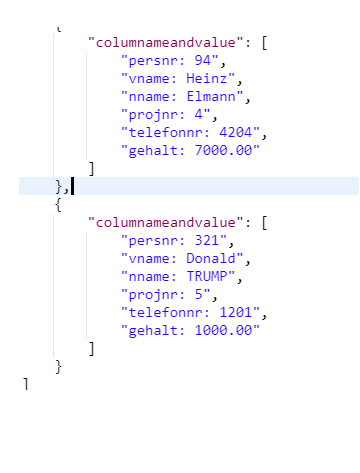
\includegraphics[width=9 cm]{Abbildungen/Insert_trump}
    	 		\caption{Gekürzte Ausgabe nach Ausführen des Befehls mit  Postman}
    	 		\label{fig:InsertQ}
    	 	\end{figure}
    	 	\newline\newline
    \noindent
    \underline{\textbf{DeleteQuery}}\newline    
    \underline{http://localhost:8001/sqlcoachservice/api/v1/dataset/1}/\newline
    \underline{execute?query=...}\newline
    Pfad Annotation: DELETE\newline
    Führt bei Aufruf die als Queryparameter beschriebene delete Query auf Datensatz eins aus. 
    Anschließend werden alle Werte der Spalte zurückgegeben, in der die Insert Query einfügte.
	\subsection{Installation}
	Voraussetzung für die Installation und Ausführung des Codes sind:
	\begin{itemize}
		\item Eine Installation von Docker 
		\item Eine Installation von Maven   (inkl. gesetzter Umgebungsvariablen)
		\item Eine Installation von JDK 1.8 (inkl. gesetzter  Umgebungsvariablen)  
		\item Eine Installation von JDK 1.8 (inkl. gesetzter  Umgebungsvariablen)  
	\end{itemize}
Das Projekt kann durch die Ausführung folgender Befehle (in dieser Reihenfolge!) heruntergeladen und gestartet werden:
	\begin{lstlisting}
	git clone git@github.com:danielbraun2019/Informatik-HS-KL-BEGGEL-SWTP-SS19_dabr1001_v2.git
	
	mvn clean package
	
	docker-compose  build 
	
	docker-compose  up
	\end{lstlisting}
	
		\subsection{Architektur}
		In diesem Kapitel wird die Architektur des Projektes beschrieben. Um diese zu strukturieren, wird diese in Reihenfolge der Installationsanleitung erläutert.
		Nachdem die Datei mit \dq git clone git@github.com:danielbraun2019/Informatik-HS-KL-BEGGEL-SWTP-SS19\_dabr1001\_v2.git\dq heruntergeladen wurde, wird mit dem Befehl mvn clean package der Code kompiliert. Maven erstellt hierbei die "war-Datei" sqlcoachservice.war, die durch die Datei pom.xml spezifiziert wurde. 
		Bei Ausführung des Befehls docker-compose build erstellt Docker die in der Datei spezifizierten Dienstleistungen (services). In dieser sind die zu verwendenden Ports, das Passwort sowie die jeweilige Dockerfile spezifiziert. Die Dockerfiles spezifizieren, aus welcher sql-Datei Daten geladen werden sollen. Des Weiteren wird spezifiziert, dass das hier erstellte Postgres-image die Skripte aus dem Dateiverzeichnis /docker-entrypoint-initdb.d/ zur Initialisierung nutzen soll.
		
		Bei Ausführung des Befehls docker-compose up löscht Docker zunächst (wie in den beiden Sql-Dateien beschrieben) alle Tabellen und Sequenzen, bevor er diese neu aufbaut. Sofern alle Tabellen und Sequenzen erfolgreich initialisiert wurden, fügt Docker die Werte aus den  Sql-Dateien in die erstellten Tabellen ein. Der Server wird nach erfolgreicher Initialisierung hochgefahren. 
		
		Wird eine Anfrage auf einer der in 3.1 definierten URL-Adresse ausgeführt, so werden die Dateien CatalogRessource.java oder PersndatensatzRessource.java initialisiert, welche einen SqlCoachDBfacet mit einer ihm zugeteilten Datenquelle initialisieren. Hikari ist für diese Initialisierung zuständig und wirft einen Fehler, wenn beispielsweise die in den proerties-Dateien spezifizierten Ports oder das Passwort nicht mit denen der docker-compose-Datei übereinstimmt. Sofern in einer der ressource-Klassen eine Methode mit entsprechender Pfad Annotation und entsprechendem Anfragetypen (Requesttyp, z. B. GET, DELETE, INSERT) existiert.
		Diese ruft dann eine entsprechende public-Methode innerhalb SqlCoachDBFacet auf. Der SqlCoachDBFacet führt dann eine Sql-Anfrage auf der zugeteilten Datenbank aus. 
		
		
		
		
		
	%------------------------------------------------
	
	\section{Diskussion}
		Fast alle  erforderlichen User-Stories wurden implementiert und wiederholt auf Funktionalität geprüft. 
		Die in der README.md nicht unter Interface Spezifikation aufgeführte User-Story der frei konfigurierbaren Datasources wurde nicht umgesetzt. 
		Datasources und Trainingsdaten müssen als Sql-Datei in das Projekt eingebunden werden und erfordern eine anschließende Konfiguration der docker-compose-Datei sowie das Anlegen von docker-und property files. 
		Alternativ können andere Datensätze in die bereits vorhandene Trainingsdatenbank kopiert und eingefügt werden.\newline
		Get Table Definitions gibt zwar die gewünschten Informationen in  JSON-Format zurück, diese basieren aber im Gegenzug zu den Get-Methoden des SqlCoachDB nicht auf Modellklassen, welche dem der zurückgegebenen Tabelle entsprechen (Scenario.java als Modellklasse zur Tabelle sc\_scenario). Sowohl die Primär- und Fremdschlüssel, als auch die Spaltennamen werden lediglich als Liste innerhalb des JSONS zurückgegeben. Vorteil dieser Implementierung ist es, dass keine IF-Abfragen oder Switch-Cases den Rückgabetyp bestimmen müssen und ebenfalls keine zusätzlichen Klassen für jede im Nachhinein eingefügte Tabellenspalte erstellt werden müssen. Statt dieser Klassen ist nur eine einzige Klasse Table\_shemas implementiert.
		Diese Designvariante wurde gewählt, weil man auf diese Weise einen kürzeren Code erhält und eine einfachere Erweiterbarkeit der Datenbank garantiert, d.h. die Methoden lassen sich auch auf anderen SQL-Datenbanken ausführen.
		\newline
		Dass bei der Programmierung auf Wartbarkeit des Codes Wert gelegt wurde, sieht man an der Implementierung der n Query-Methoden (selectQuery, insertQuery und delete Query ).
		Die zusätzlichen Methoden insertQuery und deleteQuery unterschieden sich in der ersten Version ihrer Implementierung lediglich durch den Übergabeparameter und einer verschiedenen If-Bedingung, weshalb der sich überschneidende Code in die Methode executeQueryforInsert\_Delete\_and\_Update ausgelagert wurde.  Um  dem Softwarenutzer das Prüfen der Korrektheit dieser zwei Queries zu erleichtern, geben die Methoden die veränderte Spalte der Tabelle nach Änderung aus. Diese Methode (returnColumn) ist ebenfalls ausgelagert worden, sodass der Code kürzer und wartbarer ist. Das Auslagern von mehrfach vorkommenden Code-Segmenten wurde also als Best-Practice in diesem Kontext umgesetzt. \newline 
		Bei der Implementierung der selectQuery wurde darauf geachtet, dass sie nicht nur bei einfachen Selects, sondern auch bei der Selektion von einer oder mehreren Spalten funktioniert:
			\begin{figure}[ht]\centering
			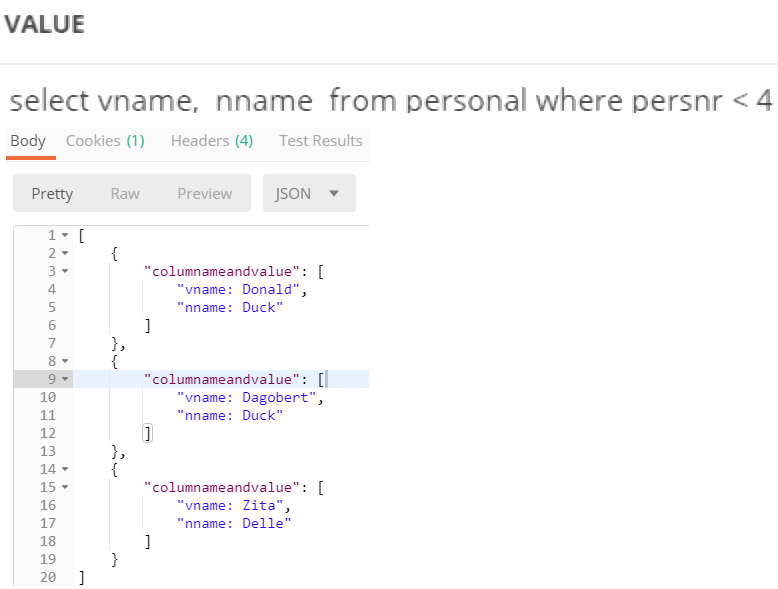
\includegraphics[width=9 cm]{Abbildungen/select_2_spalten}
			\caption{Ausgabe einer Get-Request auf de Url http://localhost:8001/sqlcoachservice/api/v1/dataset/1/execute?query=\newline select vname,  nname  from personal where $persnr \le \ $4, wobei \dq select vname,  nname  from personal where  $persnr \le \ $4\dq eine Query definiert die auf der Datenbank unter der datasetId ausgeführt wird }
			\label{fig:fsm3}
		\end{figure}
	\newline
	Die Methoden addScenario, addGroup und addExercise fügen ein Objekt des jeweiligen Datentyps in die Datenbank ein, aber setzen den aktuellen Wert der jeweiligen Sequenz als Id des Objektes. Wird beispielsweise eine  Aufgabe wie gewünscht in die als Parameter spezifizierte Gruppe eingefügt, so sind die exerciseIds innerhalb der Gruppe nicht mehr linear aufsteigend.\newline
	\begin{figure}[ht]\centering
		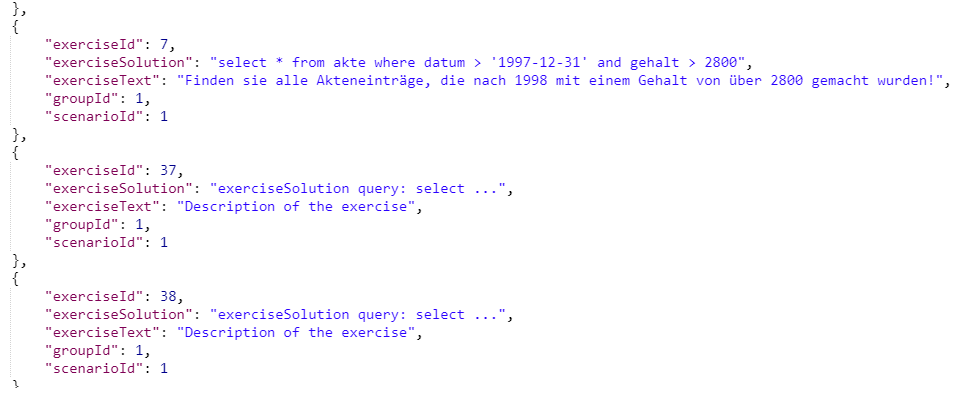
\includegraphics[width=9 cm]{Abbildungen/addExercise}
		\caption{Ausabe nach einfügen einer weiteren Aufgabe in Aufgabengruppe2}
		\label{fig:addE}
	\end{figure}
\newline
\newpage
	Es existieren keinerlei Junit-Test im Quellcode, da dieser schon während der Programmierung auf Fehler überprüft wurde. Mittels Postman und den Fehlermeldungen während des Kompilieren des Quellcodes wurden Fehler beseitigt. 
	Die Beseitigung von Fehlern während des Programmierens und der Einhaltung der zuvor erwähnten Best Practices zeigt sich bei der IntelliJ Code Inspection. Abgesehen von \dq spelling mistakes\dq werden die \dq unused properties\dq als Fehler angesehen. Diese müssen aber Maven und Docker intern sichtbar sein, da sonst der Server-start-up oder gar das Ausführen des mvn clean-package-Befehls eine Fehlermeldung geworfen hätte, weshalb diese Fehler zu ignorieren sind. 
	Außerdem findet IntelliJ nicht das Paket \dq Classfish\dq , welches aber in der Maven-Datei pom.xml aufgelistet ist und erzeugt wird.
	
	Die Schnittstellen der Anwendung sind größtenteils gut gelungen, da sie leicht verstanden werden können. Wenn man sich kurz mit der Anwendung befasst, so sollte es ein leichtes sein, zumindest GET- Anfragen auf dem Stammdatensatz auszuführen.  In diesem Kontext sehe ich es ebenfalls als vorteilhaft an, dass man hierfür nur wenige Parameter ändern muss. Die Restschnittstelle für die Methoden zum Einfügen verschiedener Szenarien, Aufgabengruppen oder Aufgaben ist meiner Meinung nach schlecht gelungen, da sie den Zusatzparameter /add hat. \footnote{Da aber das genaue Einhalten der RES-Schnitstellen Punkte gibt, wurde diese nicht verändert} Dieser Zusatzparameter ist überflüssig, weil die Einfügemethoden die einzigen Post-Requests auf der Stammdatenbank sind, sodass der Parameter nur dafür sorgt, dass mit der Konvention gebrochen wird.
		\section{Zusammenfassung}
	Programmiert wurde das Backend einer webbasierten Anwendung, welche den SQL-Coach von 2007 zum Vorbild hatte. Bereitgestellt sind Methoden zum Löschen, Ausführen, Einfügen und Updaten von Szenarien, Aufgabengruppen und Aufgaben sowie eine Stammdatenbank, in der die Szenarien, Aufgabengruppen und Aufgaben implementiert sind. 
	Darüber hinaus wurde der Personaldatensatz von Professor Doktor Schiefer in einer Weise  integriert, die es erlaubt, diese Datenbank unabhängig von den Stammdaten in einem eigenen Container auszuführen. Bereitgestellt sind ebenfalls Methoden, welche es ermöglichen, die SQL-Anfragen Select, Insert und Delete auf dem Trainingsdatensatz auszuführen.
	Auf den aktuellen Projektstand aufbauend könnte man aber auch weitere Methoden implementieren. So könnte man beispielsweise die restlichen SQL-Anfragetypen (Update, alter table, drop table etc..) einprogrammieren. Ein naheliegender Ansatz wäre es außerdem, Funktionalitäten, die im 2007er SQL-Coach vorhanden sind, aber nicht in der erneuerten Version noch in das Projekt einzubinden. So wäre es beispielsweise nötig, eine Verbindung zwischen Stammdaten, welche die Aufgabenstellung und Lösung enthalten, und der Personaldatenbank, auf der die SQL-Anfragen ausgeführt werden, herzustellen .
	Das Projekt sollte auch um ein Frontend erweitert werden, um die Anwendung für Nutzer auch ohne die Zuhilfenahme von Postman zu ermöglichen.
	Als Sicherheitsmaßnahme wäre es zu empfehlen, sicherere Passwörter in den Properties und der docker-compose.yml zu verwenden. Außerdem sollte man überlegen, ob das Ausführen von Methoden auf der Stammdatenbank/ der Zugriff zu dieser nicht nur für Autorisierte Nutzer möglich sein sollte.
	
	
	
	
	
	
	
	%----------------------------------------------------------------------------------------
	%	REFERENCE LIST
	%----------------------------------------------------------------------------------------
	
	\bibliographystyle{unsrt}
	\bibliography{Literatur}
	
	%----------------------------------------------------------------------------------------


	\subsubsection*{Erklärung zur Ausarbeitung}
	Hiermit erkläre ich, Daniel Braun (880335), dass ich die vorliegende Ausarbeitung selbstständig und ohne fremde Hilfe angefertigt habe und keine anderen als in der Abhandlung angegebenen Hilfen benutzt habe; dass ich die Übernahme wörtlicher Zitate aus der Literatur sowie die Verwendung der Gedanken anderer Autoren an den entsprechenden Stellen innerhalb der Arbeit gekennzeichnet habe. Ich bin mir bewusst, dass eine falsche Erklärung rechtliche Folgen haben kann.\\ \\
	--------------------- \\
	Unterschrift

\end{document}